\section{Aufgabe 5 - Berechnung von konvexen H�llen mit qhull}
\label{sec:Aufgabe5}
In dieser Aufgabe werden mit dem Programm \textit{qhull}\footnote{http://www.qhull.org/} zuf�llige Punktmengen erzeugt und mit diesen, eine
konvexe H�lle in verschiedenen Dimensionen berechnet.
Dabei wird zuerst ein Programm f�r die automatische Berechnung entwickelt um anschlie�end die Berechnungszeiten zu pr�sentieren.


\subsection{Programm f�r die Berechnungen}
\label{sec:programm}
Um f�r die verschiedenen Dimensionen und wechselnden Punkte die Berechnungszeiten zu ermitteln, wurde ein kleines Programm
entwickelt. Das Programm nutzt die von \textit{qhull} zur Verf�gung gestellten C++ Schnittstellen und Bibliotheken.
Die ben�tigten Bibliotheken k�nnen durch die jeweiligen Qt-Creator Projektdateien erzeugt werden.
Die Projektdatei sowie die Berechnungsergebnisse sind im Ordner \texttt{aufgabe5\\} abgespeichert.
Damit das Programm gestartet werden kann, muss es in dem \textit{qhull} Ordner \texttt{src\\} kopiert werden.
Dadurch werden alle Abh�ngigkeiten f�r das Programm verf�gbar gemacht.


\subsection{Ergebnisse der Berechnungszeiten}
\label{sec:a5ergebnisse}
In der Abbildung \ref{fig:dim2to5} werden die Berechnungszeiten f�r die Dimensionen 2 bis 5 in einem 
Koordinatensystem dargestellt. Dabei wurde eine maximale Punktemenge von $1.000.000$ zuf�llig erzeugten Punkten genutzt.
Gestartet wurde bei $0$ und schrittweise um $100.000$ Punkte bis zum Maximum erh�ht.
Die Punkte werden auf der x-Achse und die gemessenen Berechnungszeiten auf der y-Achse abgebildet.
Die Dimensionen 2 und 3 werden in der obersten und die Dimensionen 4 und 5 in der untersten Grafik gezeigt.

\begin{figure}[htb]
\centering
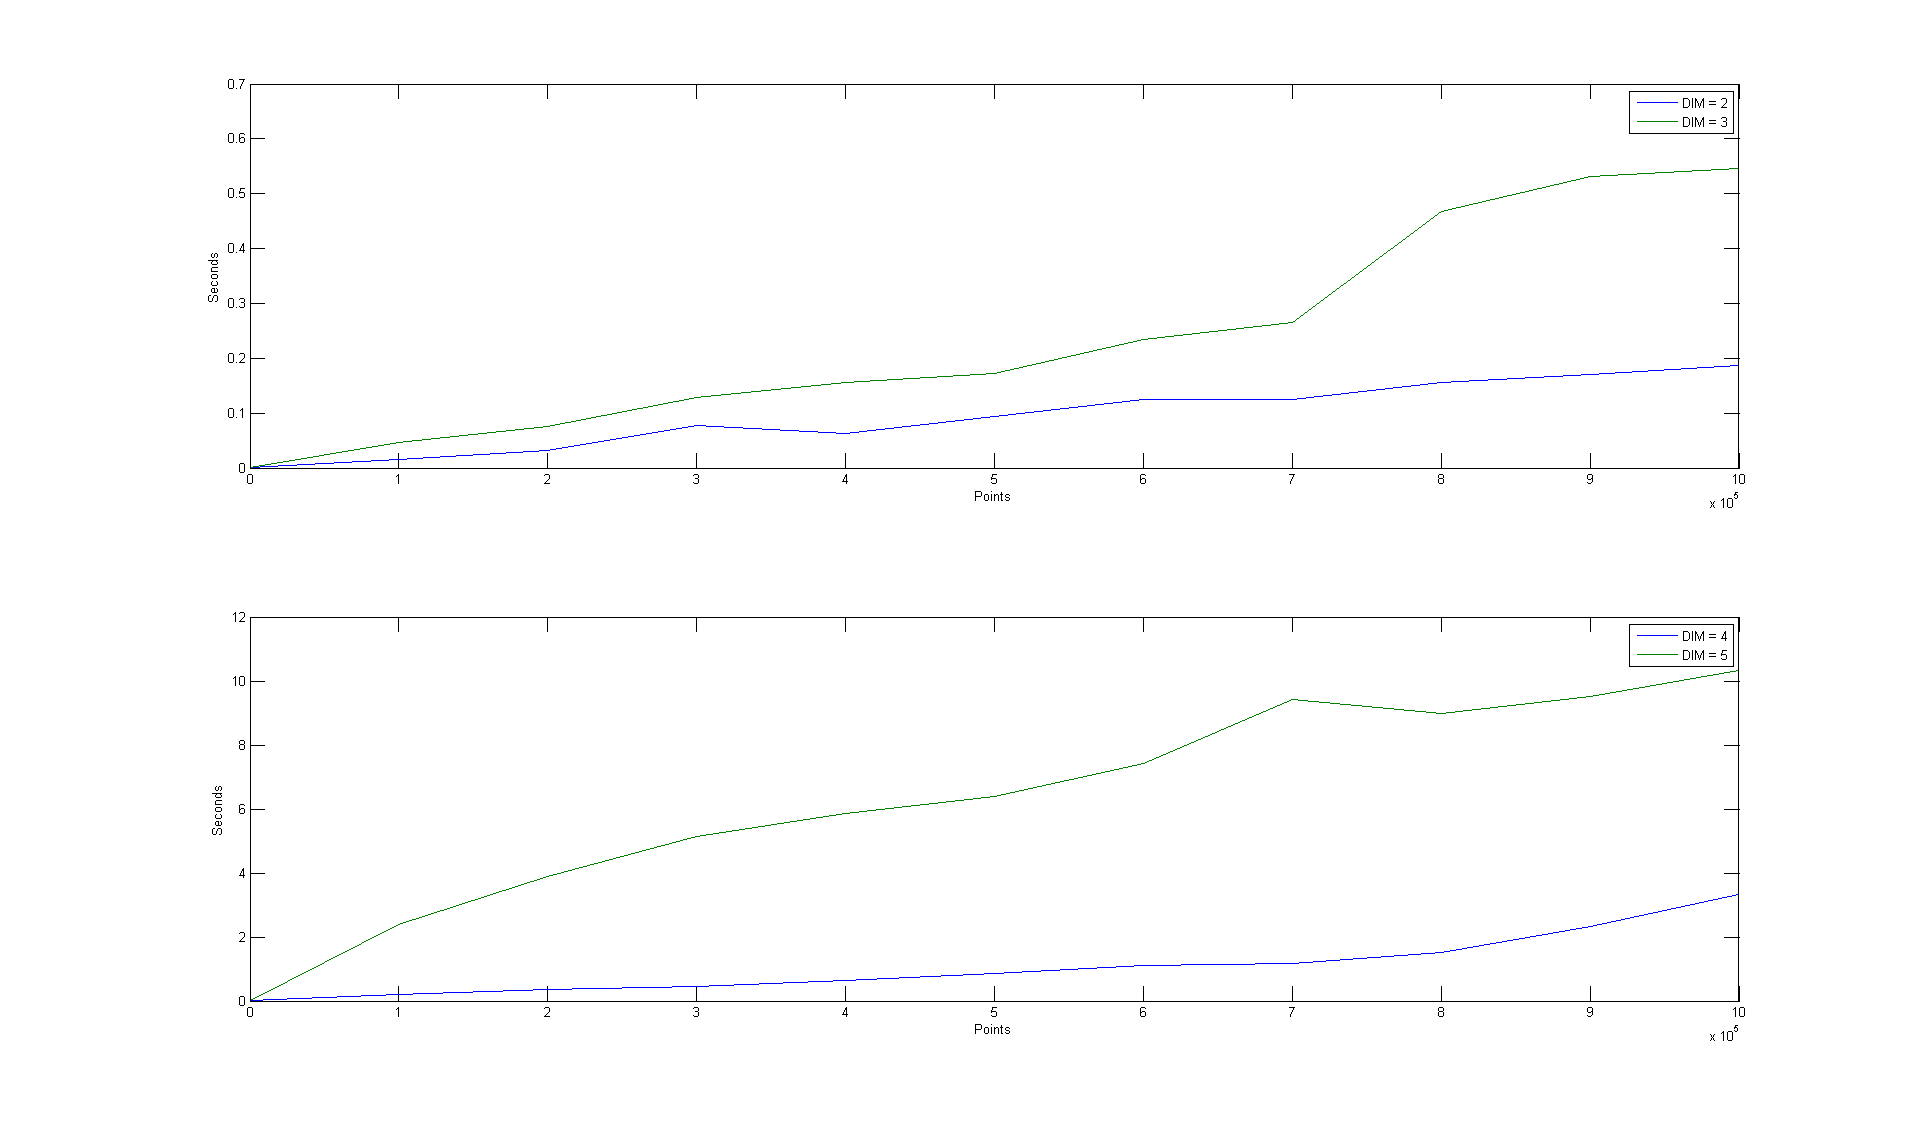
\includegraphics[width=1.0\textwidth]{dim2-5.png}
\caption{QHull Ergebnisse f�r die Dimensionen 2 - 5}
\label{fig:dim2to5}
\end{figure}

F�r die Dimensionen 6, 7 und 8 mussten die Punktemengen aufgrund von zu langen Berechnungszeiten und Arbeitsspeicher Problemen abge�ndert werden.
Die Berechnungszeiten werden in der Abbildung \ref{fig:dim6to8} in separaten Koordinatensystemen dargestellt.
Dabei wurde eine maximale Punktemenge von $1000$ Punkten mit einem Inkrementierungsschritt von $100$ Punkten verwendet. 


\begin{figure}[htb]
\centering
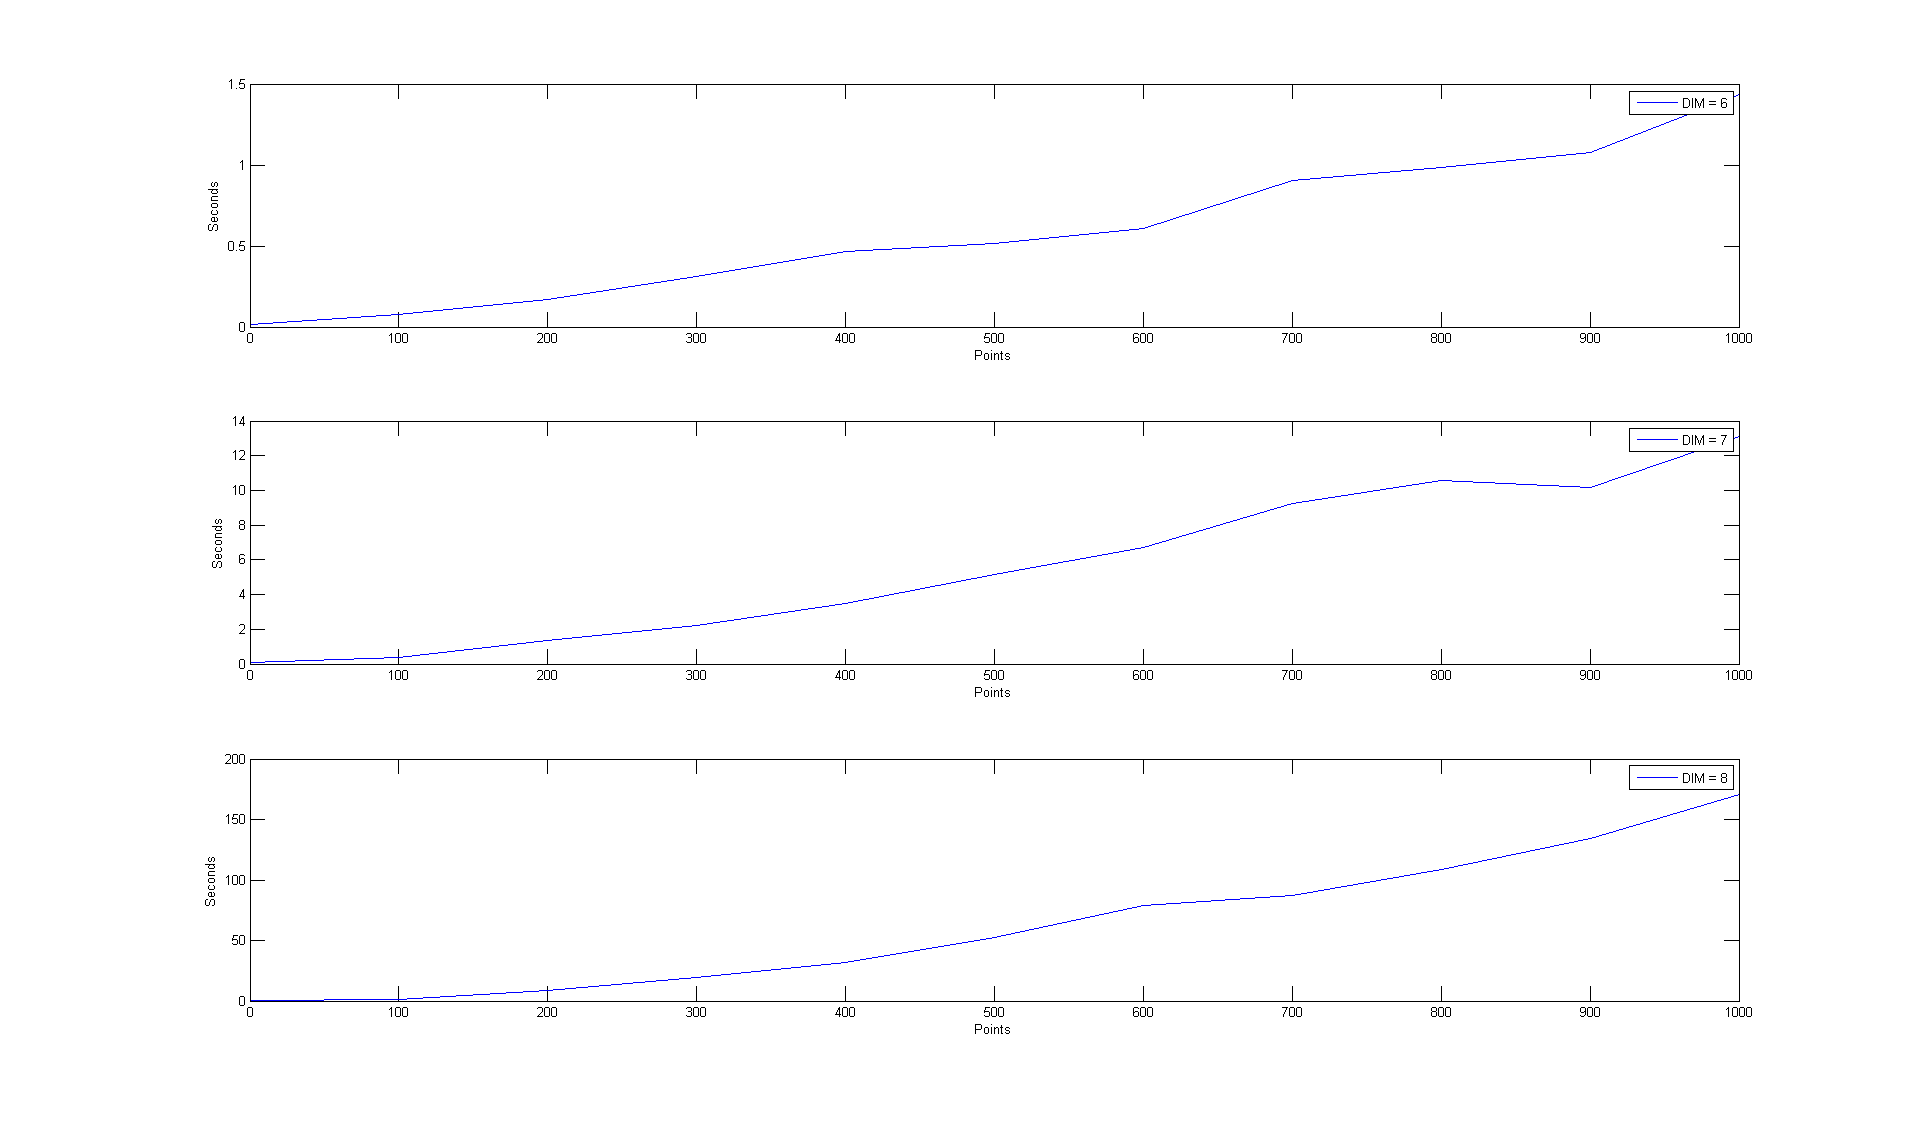
\includegraphics[width=1.0\textwidth]{dim6-8.png}
\caption{QHull Ergebnisse f�r die Dimensionen 6 - 8}
\label{fig:dim6to8}
\end{figure}